% Chapter Template

\chapter{Covariates} % Main chapter title

\label{ChapterX} % Change X to a consecutive number; for referencing this chapter elsewhere, use \ref{ChapterX}
\section{Overview}

Before we go ahead and model the relationship we have set out to explore, we must carefully set up the various covariates in our GAM. In this chapter, we will explore and justify the choice of different covariates that we use. This will allow us to standardize the model before applying it to different subgroups in the population.

\section{Covariates to Control for Differences in Population}

To analyze the relationship between the covariate under consideration and the response variable, we need to control for differences within the diverse patient cohort we have chosen for the study. Hence, in any models fitted, we control for age, gender, Body Mass Index (BMI) and maximum sequential organ failure assessment score (SOFA score). SOFA score is a score assigned to the patient to determine the extent of organ function and possibility of organ failure based on six different scores for the respiratory, cardiovascular, hepatic, coagulation, renal and neurological systems. The SOFA score allows us to control for the difference in the level of sickness between patients which affects their final outcome. More specifically, we use the maximum SOFA score of a patient as it is a good quantifier of organ dysfunction present at ICU admission \citep{moreno1999use}. 

We also note that for any controlling variable that is non-binary, there is no reason to assume that it's relationship with the response variable is linear. Therefore, for all controlling covariates except for gender (binary) we add a smoothing function in our GAM.

\section{\Sp vs SpO\textsubscript{2}/FiO\textsubscript{2}: to Ratio or not to Ratio}

One aspect of our research question is to investigate whether the SF ratio is a better predictor of mortality than \Sp. Our hypothesis is that the SF ratio captures a critical difference between patients - the level of oxygenation represented by \Fi. 

The best way to examine this is to plot the relationships between each of \Sp, \Fi and SF ratio and the probability of patient mortality as predicted by each of them. This would allow us to compare whether the trends captured by each model are the same or whether one models captures more or less of a trend. However, this direct comparison of plotted trends is not directly possible as all three metrics are on different scales, and thereby cannot be plotted on the same axis. To overcome this problem, we choose to instead plot the percentile of each of the metrics within the patient cohort versus the probability of hospital mortality and its 95\% confidence interval.  

\begin{figure}[H]
	\centering
	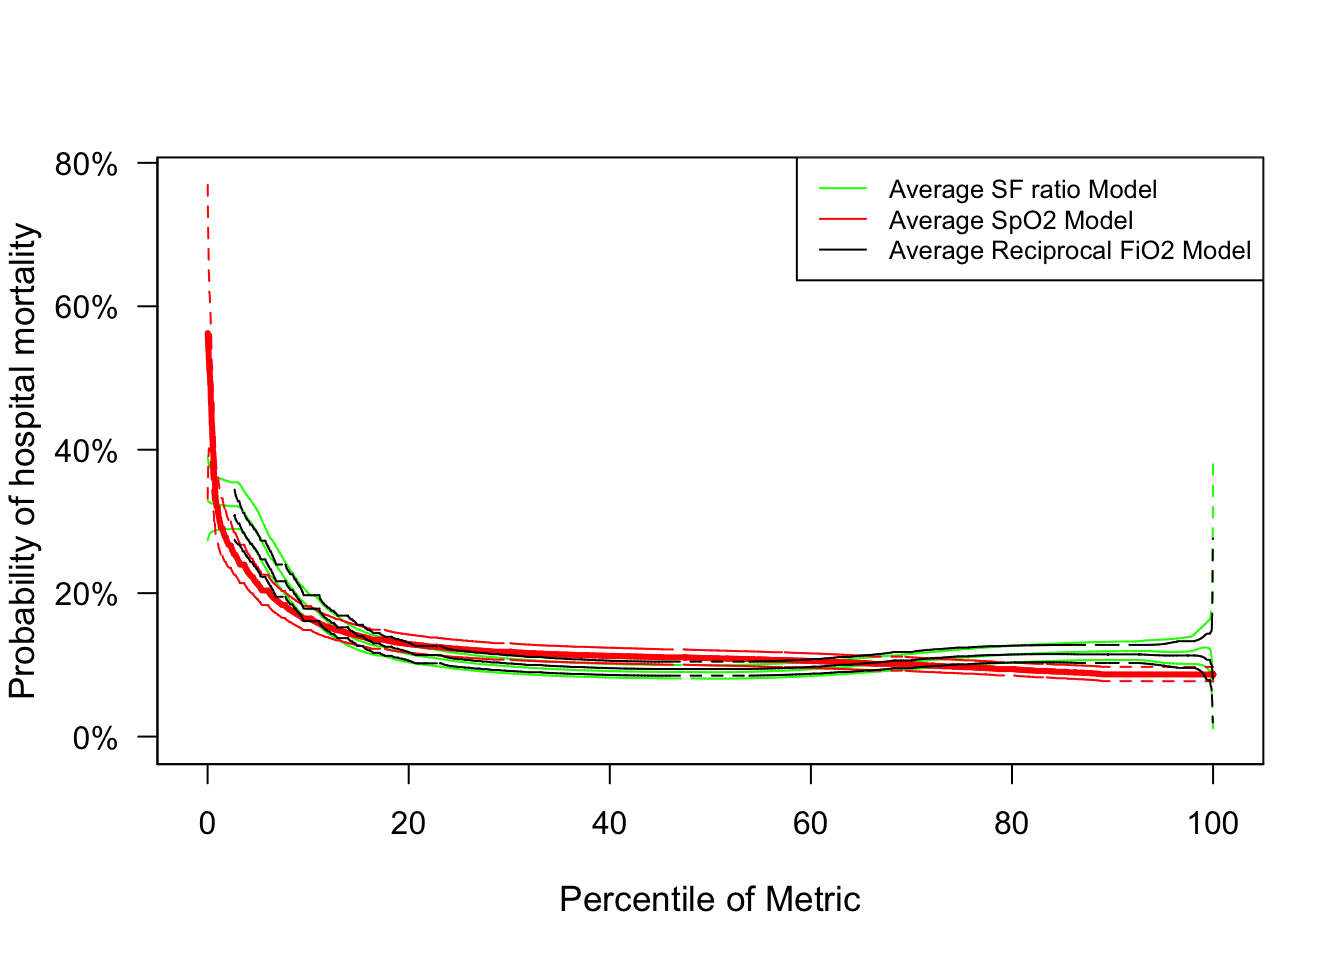
\includegraphics[width=0.9\textwidth]{figures/toratioornottoratio-4.png}
	\caption{Model Comparison: Average SF ratio vs Average \Sp vs Average \Fi}
	\label{fig:toratioornot}
\end{figure}

All three metrics are significantly correlated to patient outcome. However, as we can see from  figure \ref{fig:toratioornot} above, the SF ratio model captures both the initial downward trend of the SpO2 model and some of the upward trend towards the end  FiO2 model. Therefore, we conclude that the use of the SF ratio is better as it captures part of the unique trends of both the \Sp and \Fi. 


\section{Does Transformation help?}

In using the SF ratio however, there are two concerns. First of all, the normal range of \Fi is much wider than that of \Sp. \Fi ranges from 21\% to 100\% based on the level of oxygenation provided to the patient, while \Sp only ranges from 92\% - 100\% \citep{lapum2018vital}. In taking a ratio of these two, we are concerned that the SF ratio will be more representative of \Fi than \Sp. The second concern we have is the effect that extreme values in both \Sp and \Fi might have in increasing outlier values in the SF ratio.

To check whether these concerns are indeed an issue, we consider two different transformations of the SF ratio that tackle the two concerns respectively. We test if using them shows a difference in the trend that may not have been captured by the untransformed SF ratio. The two transformations are:

\begin{enumerate}
	\item \textbf{Linear rescaling}: We rescale both the \Sp (numerator) and \Fi (denominator) to the same scale from 1 to 2 before taking the ratio and multiplying by a 100. We shall call this the Linear Rescaled SF ratio. 
	\item \textbf{Removing Extremes}: We remove the first and last percentile of 
	both the \Sp and \Fi before taking the ratio we shall call this No-Extreme SF ratio. 
\end{enumerate} 

We again plot the percentile of each metric to the probability of mortality and its 95\% confidence interval as predicted by each model. 

\begin{figure}[H]
	\centering
	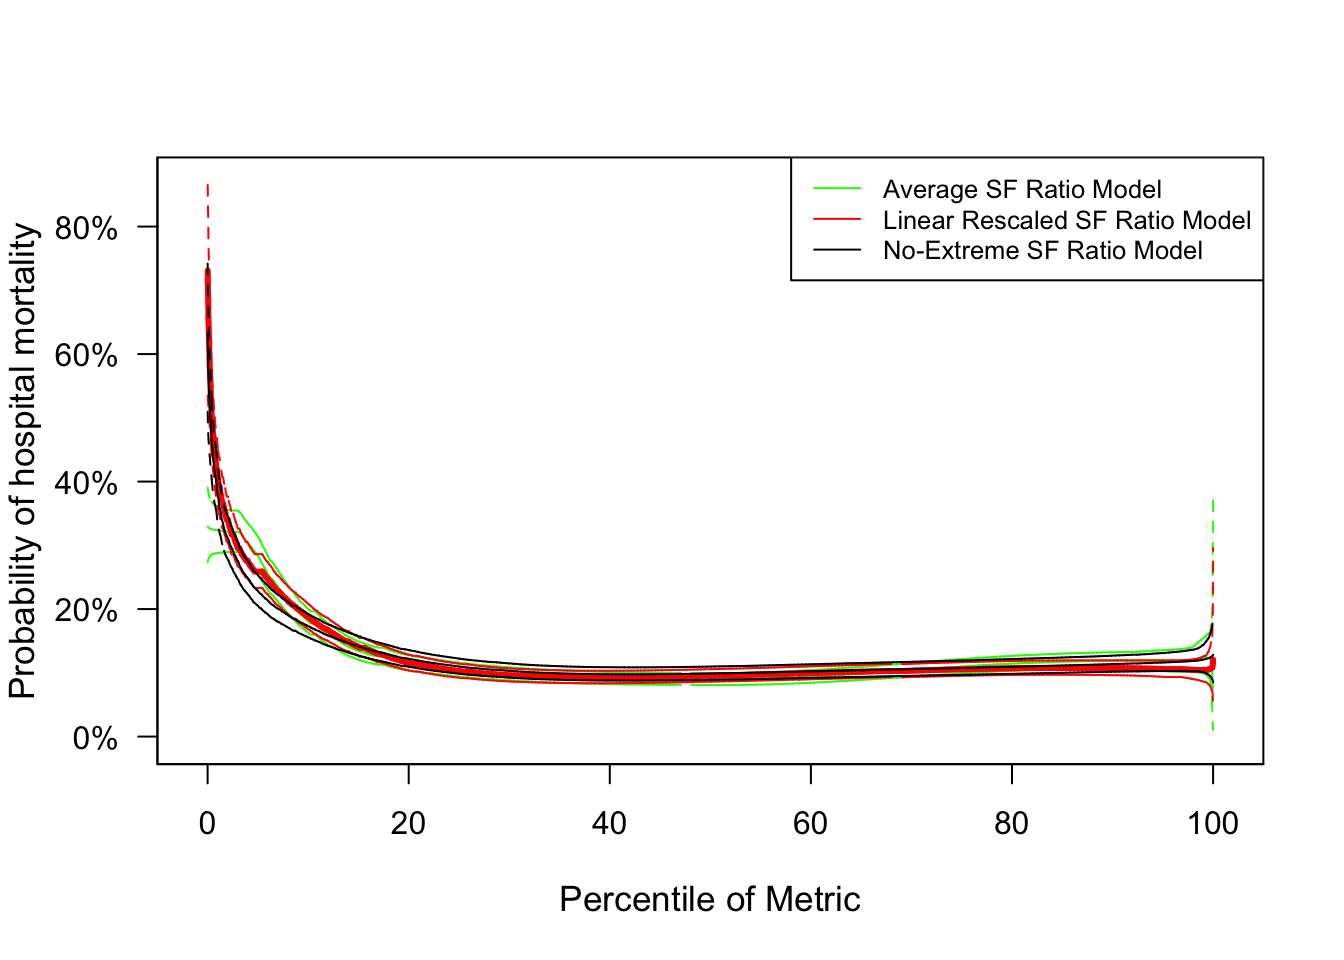
\includegraphics[width=0.9\textwidth]{figures/doestransformationhelp-4.png}
	\caption{Model Comparison: Average SF ratio vs Linear Rescaled SF ratio vs No-Extreme SF ratio}
	\label{fig:toratioornot}
\end{figure}

As the plot above suggests, all three models almost exactly coincide in predicting the confidence interval of the response variable. Therefore, it does not seem that the two suggested transformations of the SF ratio add benefit. Consequently, we will continue using the SF ratio in our models. 

\section{Time Frame of SF Ratio aggregation}

So far we have been using the average SF ratio over a patient's entire ICU stay as the main covariate in our analysis. Although significantly correlated, there lies an important drawback with this choice. The average SF ratio over the entire ICU stay can only be calculated after the patient's ICU stay is completed, which is not practical from the point of view of the intensive care specialist who is looking for an initial indicator that can help predict patient outcome. 

In this section, we shall explore two other alternative with different time frames for aggregation - the use of the average SF ratio over the first 24 hours of ICU stay and the use of the first SF ratio after ICU admission. These two alternatives are calculated during the initial part of the patient's ICU stay. If significantly correlated to patient outcome, they would be more practical alternatives to the average SF ratio over a patient's entire ICU stay. 

Below, we plot the graph between each of the covariates under consideration and the 95\% confidence interval of the probability of mortality. 

\begin{figure}[H]
	\centering
	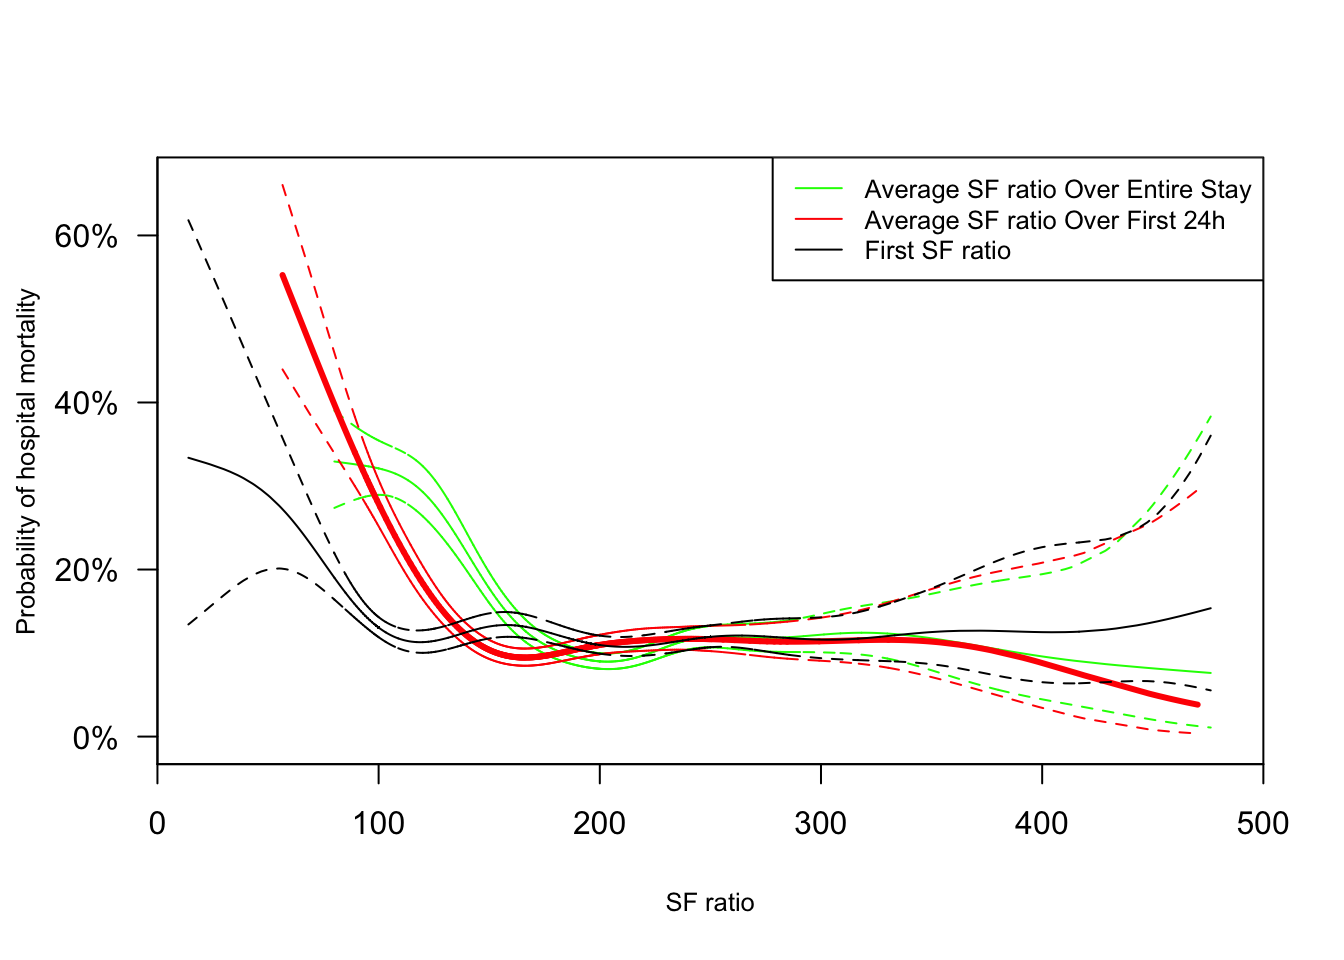
\includegraphics[width=0.9\textwidth]{figures/timeaggregates-4.png}
	\caption{Model Comparison for Different Aggregation Time Frames}
	\label{fig:timeaggregates}
\end{figure}

All three covariates are significantly correlated with patient outcome. The use of the first SF ratio model leads to wider confidence intervals than the other two, implying more uncertainty. However, this uncertainty decreases when using the aggregate of the SF ratio within the first 24 hours. Hence, the use of average SF ratio over the first 24 hours is a suitable covariate. From here on,  we shall use this instead as the main covariate in our model and refer to it as SF ratio for the sake of brevity.  

